\chapter{\iflanguage{ngerman}{Zukünftige Entwicklung}{Development}}
\label{sec:overview}

In Science Fiction Filmen wie Transcendence wird die Zukunft des Operationssaals gerne mit vollautomatisierten Robotersystemen dargestellt, die innerhalb von wenigen Sekunden sehr komplexe Eingriffe durchführen können. 
Von dieser zukünftigen Vorstellung ist die Medizintechnik noch sehr weit entfernt. Mit welchen Entwicklungen aber tatsächlich in naher Zukunft gerechnet werden kann und welche Sci Fi Ideen gar nicht so weit von der Wirklichkeit entfernt sind, soll in den folgenden Abschnitten erläutert werden.

%TODO Herausforderungen zukünftige Entwicklung und aktuell drauf eingehen
%TODO Ausblick (deshalb diese Kapitel zum Schluss)

\subsection{Neue Technologien}
Neue Technologien haben immer das Ziel, die Möglichkeiten im OP zu erweitern, mehr Sicherheit bzw. ein geringeres Risiko zu gewährleisten und das Team bei schwierigen Aufgaben zu unterstützen \cite{CurrentAndFuture}. Diese Unterstützung findet auf mehreren Ebenen statt, also nicht nur auf der Ebene der Geräte und Systeme sondern auch auf der Ebene der IT-Infrastruktur, den Funktionalitäten und der Visualisierung \cite{DerDigitaleOperationssaal}.

Geräte und Systeme die in naher Zukunft vermehrt in OP-Sälen angetroffen werden sind beispielsweise Robotersysteme. Obwohl Robotersysteme auch heute schon in der Medizintechnik eingesetzt werden, handelt es sich dabei meist um Master-Slave-Systeme, also Systeme die vom Menschen gesteuert werden. Bei sehr komplexen Eingriffen kann so eine erhöhte Präzision erreicht werden. Diese Systeme sind in vielen Fällen leider auch mit sehr hohen Investitionskosten verbunden und müssen einiger Kritik und ethnischen Fragen standhalten. Wenn Robotersysteme also regelmäßig zum Einsatz kommen, dann eher um Eingriffe durchzuführen, die ohne gar nicht möglich wären \cite{DerDigitaleOperationssaal}. Also wie beispielsweise das Operieren über natürliche Körperöffnungen. Erste Versuche in diesem Bereich wurden bereits mit dem Endosamurai (siehe Abb. \ref{fig:endosamurai}) der Olympus Deutschland GmbH durchgeführt und gegenüber derzeit verwendeter Endoskope kann man über einen Zugang Zug- und Gegenkräfte aufbringen und erreicht eine höhere Flexibilität durch bewegliche Instrumentenarme \cite{Endosamurai,DerDigitaleOperationssaal}. \\
Auch die Bildqualität von Ultraschall hat sich in den letzten Jahren enorm verbessert und aufgrund neuer Möglichkeiten wie der Aufnahme von dreidimensionalen Objekten (siehe Abb. \ref{fig:us}) in Echtzeit, findet er wieder häufiger Verwendung im Operationssaal \cite{BrainShiftInTumorResection}. Hinzu kommen Möglichkeiten zur intravaskulären Bildgebung mit Ultraschallköpfen die so klein sind, dass sie an einem Katheter befestigt werden und Bilder der Gefäßwand aufnehmen können. Der Vorteil von Ultraschall ist, dass gegenüber anderer Bildgebender Verfahren, weder der Patient noch das behandelnde Team radiologischer Strahlung ausgesetzt werden \cite{CurrentAndFuture}. Aus diesen Gründen und einer relativ guten Korrelation zwischen US-Bildern und MR-Bildern, bietet Ultraschall sehr gute Voraussetzungen um in Zukunft in der Neuronavigation Anwendung zu finden. Auch können mit Ultraschall regelmäßig intraoperative Bilder während einer Operation durchgeführt und auftretende Probleme wie Brain Shift sehr früh erkannt und darauf reagiert werden \cite{BrainShiftInTumorResection}. \\
Beim Navigationssystemen im Allgemeinen kann mit enormen Verbesserungen gerechnet werden. Neue Funktionen wie Instrumentennavigation, Kollisionswarnungen und Neuromonitoring ermöglichen strahlenfreie Mikromanipulation, Navigation und Instrumentenführung die besonders bei langen komplexen Operationsvorgängen mehr Sicherheit und Kontrolle versprechen \cite{DerDigitaleOperationssaal,CurrentAndFuture}. 

Hinzu kommt eine verbesserte standardisierte Vernetzung der Geräte und Systeme, welche die Speicherung, Verarbeitung und Übermittlung von patientenspezifischen Daten vereinfachen und herstellerübergreifende Kombinationslösungen ermöglichen. Ein übersichtliches Interface und zusätzliche Sprachsteuerung sollen zur Optimierung des chirurgischen Workflows beitragen. Und die weitere Entwicklung in der computergestützten Optimierung der Visualisierung erlaubt kontinuierliche Aufzeichnungen des Eingriffs \cite{DerDigitaleOperationssaal} und automatisierte Operationsplanung für die individuelle Anatomie des Patienten \cite{CurrentAndFuture}. 

\begin{figure} [H]
	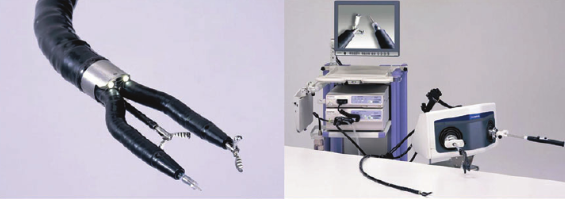
\includegraphics[scale = 0.7]{Content/Pictures/endosamurai.png}
	\caption{Endosamurai von der Olympus GmbH \cite{EndosamuraiBild}.} 
	\label{fig:endosamurai}
\end{figure}

\begin{figure} [H]
	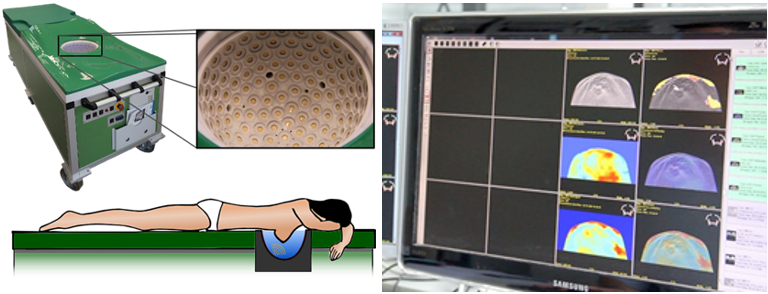
\includegraphics[scale = 0.5]{Content/Pictures/us.png}
	\caption{(Links) Wassergefülltes Untersuchungsbecken für eine (rechts) dreidimensionale Ultraschallaufnahme von der Brust zur Brustkrebsfrüherkennung \cite{Ultraschall}.} 
	\label{fig:us}
\end{figure}


\subsection{Ausblick}
Wie sich der Operationssaal zukünftig entwickeln wird und welche Technologien von den theoretisch möglichen umgesetzt werden ist abhängig von den wirtschaftlichen Realitäten. Ohne dass geklärt ist, ob die Entwicklungen tatsächlich einen medizinischen und wirtschaftlichen Nutzen in der Medizintechnik bringen werden \cite{DerDigitaleOperationssaal}, sollen ein paar Ideen genannt werden die vielleicht in Zukunft Einzug in den Operationssaal finden.

Beispielsweise könnten autonome kabelgeführte Miniroboter über einen kleinen Zugang in den Körper eingeführt werden und sich selbständig zu einer bestimmten Position im Körper vorarbeiten. So könnte der Chirurg die schwierige Navigation durch den Körper abgeben und durch den Einsatz von am Katheter angebrachter miniaturisierte Visualisierungssysteme den Vorgang überwachen \cite{DerDigitaleOperationssaal}.\\
In vielen Fällen kommt der Chirurg bei einer Operationen an die Grenzen seiner menschlichen Konzentrationsfähigkeit, da teilweise mit Händen und Füßen die medizinischen Geräte gesteuert werden müssen. Aus diesem Grund wird bereits die Sprachsteuerung integriert aber darüber hinaus ist eine Steuerung beispielsweise über die Augen vorstellbar. So könnte der Chirurg sein medizinisches Umfeld manipulieren ohne seine Körperposition zu ändern und beispielsweise bestimmte Ausschnitte des Patienten beliebig vergrößern oder verkleinern. Genauso könnte direkte Abstandsmaße von anatomischen Gegebenheiten genommen und angezeigt werden \cite{DerDigitaleOperationssaal}. \\
Eine andere vorstellbare Entwicklung könnte in Richtung eines minimierten Reinraums gehen. Dabei könnte in einer unsterilen Umgebung ein mit Vakuum fixierter Aufsatz über die Oberfläche des \glqq point of interest\grqq{} gestülpt und die Instrumente über einen Schleuse hindurchgeführt werden. Zur Umsetzung dieser Vision werden dann individualisierte \glqq single use\grqq{} Instrumente angefertigt und garantieren so eine optimale Abstimmung auf den Patienten und die Aufgabenstellung \cite{DerDigitaleOperationssaal}.

Unabhängig davon wie genau der Operationssaal der Zukunft aussehen wird, ist ein eindeutiger Trend in Richtung minimalinvasive Eingriffe zu verzeichnen. Dieser Trend wird durch die Entwicklungen in der Mikro- und Nanotechnik unterstützt und ermöglicht immer geringer belastendere Eingriffe \cite{DerDigitaleOperationssaal}.
Die Mensch Maschine Interaktion spielt eine immer wichtigere Rolle und in der Zukunft wird das Zusammenspiel aus Bildgebenden Verfahren, Navigation, Robotik, IT und Benutzerinteraktion perfektioniert \cite{CurrentAndFuture}.
Auch heute schon ist der Hybride OP-Saal die Zukunft der Chirurgie und wird sich deshalb immer weiter entwickeln, was im Endeffekt Patienten und dem Chirurgischen Team zu Gute kommt \cite{Maquet}.


	
	



